\chapter{Introduction}

\section{Scope of the Problem}\label{problem}
In 2017, breast cancer in females was estimated to be the most common cancer in the whole of Australia, and the fourth highest cause of cancer-related deaths \cite{australian_institute_of_health_and_welfare_cancer_2017}, with Australian women having a 1 in 8 chance of being diagnosed before the age of 85 \cite{australian_institute_of_health_and_welfare_breast_2012}. However with the current abilities of breast cancer screening, Australia has one of the best breast cancer survival rates, at approximately 90\% \cite{australian_institute_of_health_and_welfare_breast_2012}, where the treatment in most cases is removal of the diseased breast tissue (lumpectomy) or removal of the entire breast (masectomy), often used alongside less target-specific radiotherapy. In both cases, it is of the utmost importance for the surgeon to remove all cancerous tissue from the patient, otherwise the patient is required to undergo the surgical procedure again (a re-excision) to remove the rest of the tumour. For patients that initially underwent breast-conserving surgery in the form of a lumpectomy, most prefer to undergo a full masectomy to minimize the risk of the cancer recurring, a decision that has great significance in terms of financial cost, the cosmetic outcome, and the associated greater levels of patient anxiety. 

\begin{figure}
	\centering
    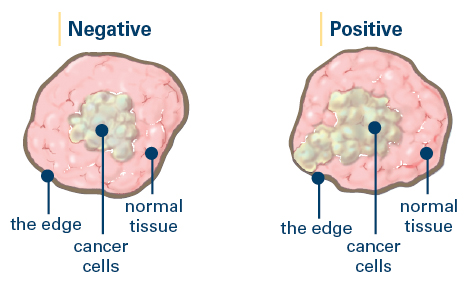
\includegraphics[width=0.6\textwidth]{bground_figs/margins.png}
    \caption{Surgical margin assessment examples of a) negative and b) positive margins. Taken from \cite{breastcancer.org_surgical_2017}}
	    \label{margins}
\end{figure}

A study in 2015 \cite{ballal_predictors_2015} found that in Western Australia, there existed a re-excision rate of 30\% for wire-guided breast conserving surgery. It is recommended that a surgical margin of 2 mm of healthy tissue be left around the excised tumour, to reduce the risk of future recurrence of cancer in the patient \cite{behm_surgical_2013}. The high re-excision rate is due to the inability of surgeons to determine whether an excised tissue has positive (cancerous tissue on the boundary) or negative (tumour-free, see \autoref{margins}) margins during surgery. The standard of care for surgical margin assessment currently is post-operative histology, which is typically available a few days after surgery \ref{allen_wide-field_2016}. The time-consuming intra-operative techniques that are currently in use (such as frozen section histology, imprint cytology, intraoperative ultrasound and specimen radiography) still report high position margin rates \cite{cabioglu_role_2007}. Use of an imaging method capable of examining excised tissue boundaries (or even tissue boundaries within the breast cavity itself) with high specificity and sensitivity during surgery would likely decrease this re-excision rate \cite{ballal_predictors_2015}. The section below describes one possible imaging method that could be used to address this problem. 

\section{Elastography}\label{elastography}
Elastography measures the deformation of tissue in response to an external mechanical load, which is used to produce images of mechanical contrast, such as the stiffness (elasticity) of the tissue, or the strain induced within it. Cancer pathology changes the mechanical properties of tissue: regions of tumour are stiffer in comparison to softer, healthy tissue \ref{fung_biomechanics_1981}. The sense of touch used by a surgeon to differentiate tumour from healthy tissue is analogous to elastography on a much coarser scale. 
Elastography was developed to enable quantitative, more accurate images of these mechanical properties of tissue to be formed. The technique operates by utilising an underlying imaging system to record the changes in different tissues in response to an applied mechanical load. The technique was first developed using ultrasound to record the reflection of sound waves before and after loading \cite{ophir_elastography:_1991}, but has since been extended to other modalities. The use of optical imaging techniques as underlying imaging tools for elastography allow much higher resolution imaging in comparison to existing clinical modalities such as ultrasound or X-ray imaging, enabling access to the mechanical properties of tissues on the micrometre scale \cite{schmitt_oct_1998} \cite{kennedy_review_2014}.
These maps offer insight into the study of disease at scales varying from organs to tissue micro-architecture, which can be probed by utilising different imaging techniques to investigate the deformation of the tissue.

\section{Optical Coherence Elastography}\label{solution}
\begin{figure}
	\centering
    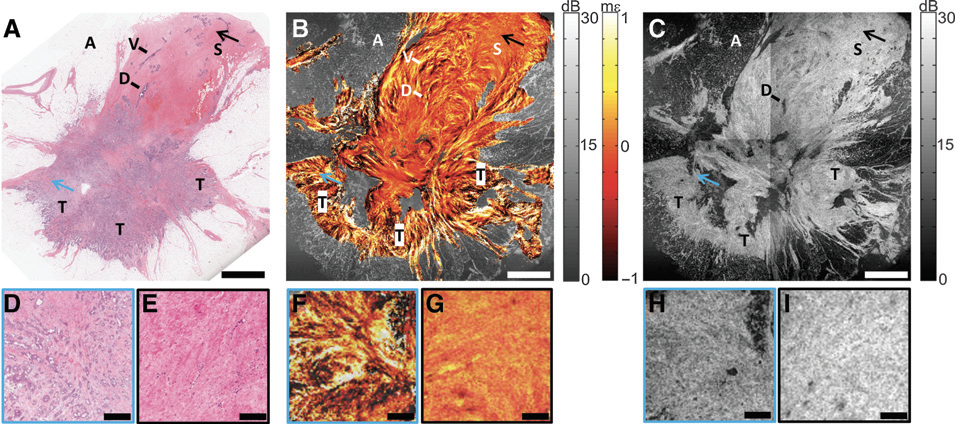
\includegraphics[width=\textwidth]{bground_figs/oce_example.png}
	\caption{An example \ac{oce} image of breast tissue, taken from \cite{kennedy_investigation_2015}. B,F and G show strain elastograms, C, H and I the \ac{oct} images. Below the main images, magnified regions of tumour (D,F and E as indicated in A, B and C) and healthy tissue (E, G and I, corresponding to the regions indicated by the arrows in A, B and C) are presented side-by-side for contrast for each imaging technique.}
    \label{oce_example}	
\end{figure}

Elastography techniques commonly used with optical imaging modalities can be thought of in three categories: compressive, resonant and shear wave based elastography. Static or quasi-static methods of loading include compressing the tissue, either through an indentation point or in bulk, and measures the resulting deformation of the tissue by detecting the displacement field produced between two image acquisitions \cite{kennedy_optical_2014}. This displacement can be used to calculate the local strain at different points in the image, which is inversely related to elasticity. Resonant loading methods, that impart a step or continuous wave loading using a range of forces (including acoustic, magnetic, photothermal, physical, among others), and can record the natural frequency of the tissue, the square of which is directly proportional to elasticity \cite{kennedy_optical_2015}. Shear wave techniques use the phase velocity of a propagating wave within the tissue as a mechanical contrast parameter, as generated by a pulsed or periodic load. 

\ac{oce} utilises \ac{oct} as the underlying imaging technique. \ac{oct} relies on the optical properties of tissue to generate contrast in an image formed by backscattered light, and can be thought of as the optical analog to ultrasound imaging. The significance of \ac{oce} lies in its ability to provide high resolution images at low sample depths. These properties differentiate it from other elastography techniques, such as those based on ultrasound, which could be used to image deep within the body due to the higher penetration of sound waves into tissue, but only at a much lower resolution due to the size difference between acoustic and optical waves. An example of \ac{oce} imaging is shown in \autoref{oce_example}. The ideal application of \ac{oce} is at surface tissue (such as imaging the retina, or skin \cite{kennedy_review_2014}), on excised tissue in a surgical setting, or used as a tool during surgery on uncovered tissue. The third application forms the main motive for this project.

Improvements to \ac{oce} system hardware and protocols have allowed scanning of entire lumpectomy surfaces in under 20 minutes \cite{allen_wide-field_2016}. To be able to provide \ac{oce} images within intra-operative time frames during surgery, the processing of the optical data from the \ac{oct} system to produce elastography images must also be done this rapidly. Essential in this processing for many \ac{oce} techniques is the computation of the local strain within the tissue from the measured deformations. 

\section{Project Aims}\label{aims}

The current OCE processing algorithm used by \ac{britelab} involves 3-D phase unwrapping to determine the axial displacement, followed by a weighted least squares linear regression estimator to calculate the axial strain. Both these steps are time consuming, and a barrier towards intra-operative imaging, which would require strain computation times of less than 5 seconds. The purpose of this thesis is to investigate techniques of speeding up the processing of strain in phase-sensitive compression \ac{oce}, for the purpose of real-time surgical application in breast cancer surgery. This is achieved through the following approach:
\begin{enumerate}
	\item Implement six different strain estimation algorithms, characterised by their phase unwrapping techniques and strain differentiation filter.
	\item Optimise the processing speed for these algorithms.
	\item Implement techniques towards maintaining image quality for rapid strain estimation algorithms.
	\item Produce arguments for an optimum strain estimation algorithm for intra-operative imaging of tissue.
\end{enumerate}
The goal is to compare strain estimation techniques on a tissue-mimicking phantom using metrics of processing time (as an indication of its ability to be extended to intra-operative imaging) and sensitivity (to monitor image quality). Once these parameters are optimised, the resulting image resolution is investigated as a measure of the ability to detect object boundaries in strain elastograms. Maintaining high image quality while implementing rapid processing techniques in \ac{oce} strain estimation is a strong step towards the goal of applying \ac{oce} imaging to intra-operative assessment of breast cancer margins, and hopefully resulting in reduced re-excision rates for breast cancer patients. 
